\documentclass[runningheads]{llncs}
\usepackage{llncsdoc}
\usepackage{makeidx}

% ~~~~~~~~~~~~~~~~~~~~~~~~~~~~~~~~~~~~~~~~~~~~~~~~~~
% Preamble: Packages required for the paper
% ~~~~~~~~~~~~~~~~~~~~~~~~~~~~~~~~~~~~~~~~~~~~~~~~~~
\usepackage{graphicx}
\usepackage{multirow}
\usepackage{epstopdf}
\makeindex
% ~~~~~~~~~~~~~~~~~~~~~~~~~~~~~~~~~~~~~~~~~~~~~~~~~~


\begin{document}

\title{Evolving Motion Machines}

\author{Nathan Douglas\\10160679}


\institute{ 
\email{nathan.douglas@ucalgary.ca}
}

\maketitle

% ~~~~~~~~~~~~~~~~~~~~~~~~~~~~~~~~~~~~~~~~~~~~~~~~~~
% ABSTRACT
% ~~~~~~~~~~~~~~~~~~~~~~~~~~~~~~~~~~~~~~~~~~~~~~~~~~

% \begin{abstract} 
% Describe in one or two sentences what your project is about.
% \end{abstract}

\section{Introduction}
\label{sec:Introduction}
Emergent computing has been previously used in many areas before.
In particular, the iterative approach taken by both evolutionary and genetic systems has repeatedly proven its' ability in several domains.
The gradual approximation technique for a given goal function can create very interesting, efficient, and effective solutions.
Further, some implementations have been remarkably effective in modelling real world behaviour.
With each implementation and domain being so unique, there exists plenty of room for continued application of these techniques.

This research aims to expand on the existing pool of implementations using emergent approaches.
General approaches are designed to either recreate natural behaviours or search for new optimal policies.
This is done first by creating a proposed solution, or genotype, with some initial value selected for each variable part of the solution.
The genotype or genotypes are then implemented and become their resulting phenotypes, which are then evaluated.
Finally, the genotypes which created the most effective phenotypes are mutated slightly, and repeat the process of instantiation and evaluation.
This creates the iterative process of searching for better and better solutions to a given goal function.

However, most research surrounding emergent computing is more focused on behaviours.
The structure of the phenotype is generally static, while the actions and reasoning are given more careful attention.
This system looks to use evolutionary strategies in a different way, focussing more on the resulting structure of a solution.
To this end, a rather simple goal function is used: simply move as much as possible.
The more complex aspect is in the genotype's large influence over the structure of the agent it generates.

Agents in this system are created from small, atomic pieces that join together to create larger collective structures.
Atoms have different simple geometric shapes, different types of motion, and a variable direction and intensity of the motion.
While atoms can mutate this direction and intensity as part of their evolutionary loop, they can also mutate additional adjoining atoms.
These new pieces attach to their parent using a physical link, creating a large branching tree structure.
With each atom still moving independently, this creates large agents with many independently moving subtrees.

This high degree on independence between subtrees creates a very dynamic structure with many different potential solutions.
Ideally this variability allows for interesting results.
As with evolution in nature, this system intends to mimic the variation in structure of life on earth.
As is shown below, this goal is somewhat met but the system itself is still too premature to be a comparable analog to natural selection.

\section{Implementation}
With the goal of moving as far as possible in each generation, an appropriate environment is needed to evaluate in.
Further, within the environment there are a list of features that must be included to support the evaluation.
First and foremost is the ability to deserialize a given genotype into a phenotype, or agent, to be evaluated.
Also needed is the inverse serialization ability.
Then, agents need some physics simulator to operate within and source the evaluation of exactly how much distance has been covered.
To this end, the Unity Engine is used as it provides a simple object instantiation scheme and a built-in physics simulation engine.

\subsection{Phenotypical Agent Structure}
Unity's simple object instantiation scheme is used to create the agent's constituent atoms.
Unity contains simple geometric shapes including spheres, cubes, and capsules.
Atoms can be one of these three shapes, which are scaled individually to make all atoms approximately the same size.
The scaling factor is different for each shape, as the shapes are different sizes by default.
The factor is set such that each shape has no cross section with a width larger than 1 meter as defined by Unity's measurement system.
This way, adjacent atoms can be instantiated 1 meter apart and do not overlap, as overlapping objects cause unexpected behaviour in the physics simulation.

Agents themselves are collections of these atoms.
Specifically, an agent is a 3-dimensional cubic grid, where each item in the grid can be either an atom or simply empty.
Atoms adjacent to each other within the grid can be physically linked to each other with invisible joints. 
These joints force the two connected atoms to be a static distance apart, mostly restriciting them from moving either closer or further apart.
The distance between two joined atoms is not completely static though, as Unity's physics engine allows the joints to stretch, compress, and bend to a small degree.

Each individual atom may either remain static or rotate around the center of its space in the grid.
This is the main way that an agent is able to move, outside of gravity causing an unbalanced agent to topple.
Further, the joint based structure combined with individual atom rotations allows for complex agent movement.
A rotating atom attached to another atom causes the attached atom to leave it's initial space in the grid and orbit the rotating atom.
Intuitively, this works like a fan.
A center piece rotates in place, and the blades are forced in a cyclic motion around the center.
The direction and force of rotation varies between atoms, with direction also controlling orientation for both static and non-static agents.

\subsection{Genotypical Agent Structure}

The genotypical structure of agents is very similar to the phenotypical instantiation.
Agents are stored as 3-dimensional arrays with each index containing specific data about its corresponding atom.
Each atom is stored as a simple collection of four values; 
two integers for the shape and motion types, a float for the motion's force, and a vector containing the rotation direction.

Agents are structured this way partly because it makes serialization and deserialization simpler.
Serialization of agents converts the array of atoms into one long string.
First, atoms are serialized using Unity's built in serialization tools which simply convert the four fields described above into json format.
The array is then flattened to a 1-dimensional equivalent.
Each atom's json representation is then added to the agent's total serialized format, using semicolons to delimit the json strings.
Deserialization simply reverses this process, retrieving the necessary information for each atom from the serialized string.

The major reason for structuring agents this way is that it is simpler to create the phenotype given this representation.
Stored as an array, detecting conflicting atoms is as simple as checking the index in question.
This is crucial for agents that modify their own structure, as is outlined in 2.3.
It is also a very simple representation to work with, although it does require more space than is aboslutely necessary.
However, alternative approaches to indexing spaces in the array that also determine conflicting neighbours in 3-dimensions adds unnecessary complexity to the structure.

Within the array, atoms are joined in a tree-based structure.
Each agent has exactly one atom that is not joined to a \textit{parent} atom, essentially creating a root node.
This root node can then be joined to each atom in its von Neumann neighbourhood.
These \textit{children} can then further join to atoms in their neighbourhood, excluding their parent.
The joints used work similarly to ball and socket joints, allowing full rotation around any axis but keeping distance between each atom constant.
Thus a \textit{parent} atom applies rotational force to its \textit{child} atoms, but not vice versa.
This tree structure acyclically joins all atoms together, creating a single large agent.

\subsection{Mutation System}
This system mutates agents in two primary ways.
First are \textit{Point Mutations} which modify the details of a particular atom.
Second are \textit{Expansions} which control the creation of new atoms as part of the agent.
Both mutations may apply to each atom at a given rate.
There are seperate rates for point and expansion mutation which do not change over the system's runtime.

Point mutations are relatively simple.
If an atom is to be mutated, another random decision is made on which field is changed; either shape, motion, force, or direction.
Each field is equally likely to be mutated, given the atom has been selected to mutate.
Shape and Motion mutations simply select a different, random element from the set of possible values.
Force is modified by a static delta which is equally likely to be added or subtracted from the force's current value.
The possible values for the force are bounded by zero and another static maximum force parameter.

Mutations to the atoms direction are more complicated however.
Similar to how force changes, direction is modified by either adding or subtracting a static delta.
This delta applies independently to each axe, and each axe may or may not rotate for any given point mutation.
For example, one direction mutation may cause the atom to rotate around the x and y axes but not the z, while another rotates only around the z.
A directional mutation must cause at least some rotation though.

Expansions control how the agent can change its overall structure over time.
If an atom is selected to expand, one of the atom's von Neumann neighbours will be checked for an existing atom.
If an atom exists in the index checked, the expansion will fail and no mutation will occur.
Otherwise, a new atom will be generated at random in that location, with the new atom being joined as a child to the mutated atom.

\subsection{Evaluation System}
A proper goal function to optimize is critical to any evolutionary system.
Agents in this system are given the goal of traveling as far from their initial position as possible in each generation.
Generations are bounded by a generation length parameter that determines how much time agents are given within a generation to produce movement.
Four agents are run in parallel, set not to collide with each other, and the agent that travels the greatest distance in that time is used to seed the next generation.
Initially, agents consist only of their root atom and a single random child.
Any further variations are caused by the evolutionary system.

Determining distance is a non-trivial task however.
This system interprets distance as the amount of distance travelled by the root atom of that agent.
While all the pieces of an agent can move in space, only changes in the root atom are recorded.
This calculation is performed by summing the change in global position of the root atom in every frame of the physics simulation.
This includes motion in all three axes, and thus includes motion types such as spinning, shaking, and rolling.

\section{Results}
\begin{figure}
    \begin{center}
    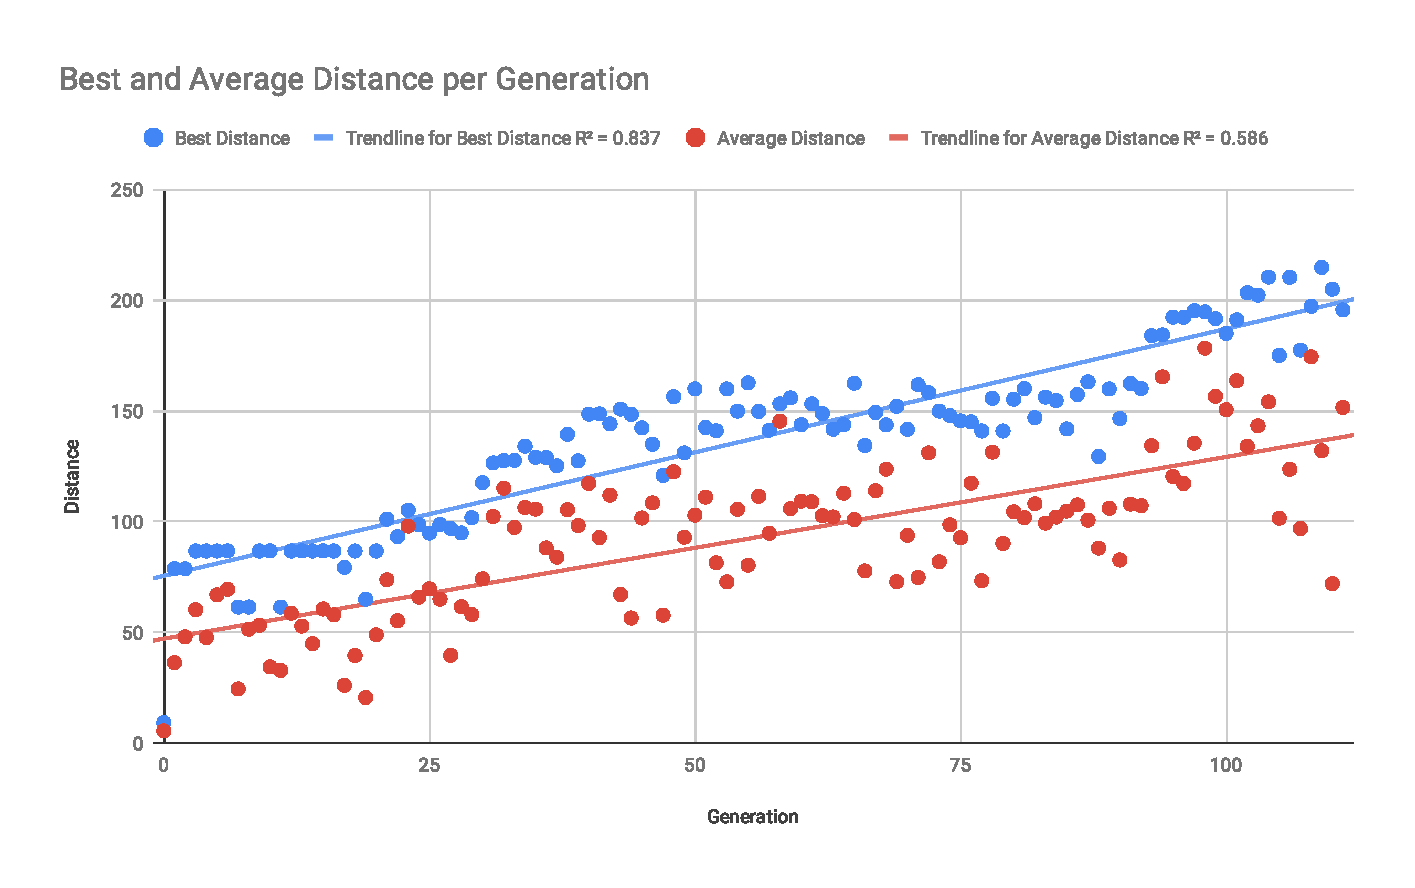
\includegraphics[width=1\textwidth]{DistanceChart}
    \end{center}
    \caption[ ]{
        A scatter plot showing both the best and average distances in meters achieved in each generation, as well as a trend line for each metric.
        The variance in the best distance attained is a product of Unity's physics engine being non-deterministic.
    } 
    \label{fig:DistanceChart} 
\end{figure}

Before fully discussing the specific results of the system, two major caveats need to be discussed.
First is that the system, by design, has an incredibly large search space.
The intention was to create a system that has significant variance in the agents it produces.
The consequence, however, is that finding the global optimum is nearly computationally impossible.

This issue is further exacerbated by the following, more difficult problem.
This experimentation has shown that Unity's physics engine is not deterministic, which creates difficulties in evaluating the performance of an agent.
Using the default settings provided in the simulator, significant variance can be observed in the outcome of even simple physics tests such as dropping an object on the ground.
For large, complex agents, this variance expands exponentially and can cause an effective agent to fail when re-evaluated.
This behaviour was not noticed until observing the thrashing of best results visible in Fig. 1.

To address this issue, the simulation's settings were increased to best performance.
This somewhat alleviated the issue, but results still varied.
The results shown in Fig. 1. use the optimized settings, but the thrashing is still very apparent.
This also incurred a significant performance penalty, such that even slightly outdated computers may experience slow down.

However, even with this thrashing behaviour occuring the system provides positive results.
Distance covered trends upwards at a fairly linear rate throughout the system's lifetime.
Most improvements make simple point mutations to a small number of atoms, slightly increasing the agent's overall performance.
Others cause significant vertical jumps in the agent's performance and are usually caused by a significant change in structure.
Overall, despite the thrashing that is pervasive in the results, agents do successfully grow both in structure and performance.

The actual structure generated by agents tends to fall into to main categories.
Agents in the first category have 2-4 long, mostly static branches which jut out from the agent's root atom. 
These branches swing around wildly, causing the agent to jump and bounce in a mostly random fashion.
In the second category, agents make large flat spinning discs.
These discs are imbalanced, such that the whole rolls on the edge of the disc approximately 20 degrees off the ground.
Most of the time, agents in the second category look like off-balance wheels, while the first look like flailing arms and legs.

These results are very strong indicators that this system is working as intended.
This system does seem to favour larger, more complex agents rather than simple agents that use a simple motion type.
Further, the abstract shape of agents that emerges is surprisingly rational very frequently.

\section{Future Work}
While this system is a very positive result, there are many ways in which the system can be improved.
First and foremost would be to increase the number of motion types available.
Atoms can currently either rotate or not move at all, but a linear thrusting type of motion may increase the number of different types of agents.
Another approach would be to allow cyclic joints in the agents structure, creating larger, stronger structures from the base atoms.
Finally, by using the agent's center of mass to measure distance, the thrashing behaviour may be addressed further.

There are also other potential extensions of the system thtat might be of benefit that do not require changing the agent's structure.
First would be to modify how distance is measured.
Many agents in the current system abuse the cyclic motion types to spin in place or roll in small, tight circles.
To address this, a distance measurement that penalizes angled movements may create different overall behaviours.
By penalizing angles, rather than jumping and spinning agents would likely learn to move in continuous straight lines.

Another approach would be to introduce varied terrain, rather than the current terrain that is simply a large, flat plane.
Contrary to the approach above, introducing hills and valleys may cause vastly different behaviour.
It's difficult to determine whether the same structures generated for this terrain would work for terrains.

\section{Conclusion}
This system has shown strong results while taking a less common approach to evolutionary systems.
The two research goals, creating several diverse solutions and creating complex moving structures, have both been met.
However, the system is still clearly in an infantile state, and there is lots of room for improvement.
This is yet another positive for this system, as further development is likely to produce more and more interesting results. 

\end{document}